% ---------------------------------------------------------------------------- %
\chapter{Fundamentos}
\label{cap:fundamentos}
% ---------------------------------------------------------------------------- %

Para se criar e treinar uma inteligência artificial, diversos arcabouçous são necessários. Por um lado, existe a parte teórica e matemática na qual a inteligência se baseia para aprender. Por outro, do lado computacional, existem as bibliotecas que auxiliam no desenvolvimento, efetuando as contas necessárias e, neste trabalho em particular, emulando o jogo que serve de ambiente para o aprendizado.
Este capítulo tem o intuito de familiarizar o leitor com a teoria e as ferramentas utilizadas no treinamento da inteligência artificial deste trabalho.

% ---------------------------------------------------------------------------- %
% https://en.wikipedia.org/wiki/Asteroids_(video_game)
% https://en.wikipedia.org/wiki/Golden_age_of_arcade_video_games
% https://www.arcade-museum.com/game_detail.php?game_id=6939
% https://www.ranker.com/list/the-most-popular-golden-age-arcade-games/video-games-lists
\section{\textit{Asteroids}}
\label{sec:asteroids}

\textit{Asteroids} é um jogo de fliperama do gênero shooter (jogo eletrônico de tiro) lançado em novembro de 1979 pela então desenvolvedora de jogos eletrônicos Atari Inc, atualmente conhecida apenas como Atari. O jogo foi inspirado por \textit{Spacewar!}, \textit{Computer Space}, \textit{Space Invaders}, e \textit{Cosmos}, sendo este último um jogo não finalizado.

O jogador controla uma nave espacial que se encontra em um campo de asteróides e precisa atirar para destruir todos enquanto evita colisões com os mesmos. A dificuldade aumenta conforme o número de asteróides na tela aumenta.
Diversas versões deste jogo foram criadas ao longo dos anos. Além das diferenças gráficas, as mudanças incluem naves espaciais inimigas que atiram contra o jogador, e tamanhos e formatos diferentes que os asteróides podem ter.
\textit{Asteroids} é considerado um dos primeiros grandes sucessos da era de ouro dos jogos de fliperama, época em que os jogos eletrônicos se estabeleceram como uma força dominante na cultura popular. 

Para este trabalho, \textit{Asteroids} foi emulado utilizando a plataforma Gym-Retro da companhia de pesquisas de inteligência artificial OpenAI. Todas as informações sobre o jogo apresentadas a seguir referem-se a tal versão.
Para o aprendizado da inteligência artificial, não há naves inimigas e os asteróides podem assumir três tamanhos e três formatos distintos. Os tamanhos são grande (inicial), médio e pequeno, enquanto os formatos são consideravelmente parecidos.
Há cinco comandos disponíveis: mover-se para frente, girar a nave no sentido horário, girar a nave no sentido anti-horário, atirar para frente, e entrar no hiper espaço. Mover-se para frente e girar no sentido horário ou anti-horário são as principais formas de movimento disponíveis ao jogador, e atirar serve para destruir os asteróides. Mover-se no hiper espaço consiste em fazer a nave desaparecer e, depois de alguns instantes, reaparecer em um local aleatório da tela. Há o risco de reaparecer em cima de um asteróide e, com isso, ter a nave destruída e perder uma vida.
A nave possui aceleração e desaceleração - ou seja, inércia. Em outras palavras, mesmo que o jogador deixe de pressionar o botão de mover-se para frente, ele continuará em movimento por um curto período de tempo antes de parar por completo. Isso gera um grau a mais de complexidade, pois faz com que manobras de esquiva e curvas sejam mais difíceis de serem devidamente executadas.

% ---------------------------------------------------------------------------- %
% https://github.com/openai/retro
% https://blog.openai.com/gym-retro/
% https://openai.com/
% https://gym.openai.com/
\section{Gym-Retro}
\label{sec:gymretro}

Gym-Retro é uma plataforma para pesquisa de aprendizado por reforços e generalização em jogos desenvolvida e mantida pela empresa de pesquisas em inteligência artificial OpenAI. O lançamento mais recente inclui, como ambientes para o desenvolvimento de IA, jogos do Sega Genesis, Sega Master System, Nintendo Entertainment System (NES), Super Nintendo Entertainment System (SNES) e Nintendo Game Boy, além de suporte preliminar para Sega Game Gear, Nintendo Game Boy Color, Nintendo Game Boy Advance e NEC TurboGrafx. Em qualquer um desses consoles, a ROM (Read Only Memory) do jogo é necessária.
Apesar de não ter sido utilizada neste trabalho, a plataforma disponibiliza uma ferramente que permite criar save states (salvar um estado a partir do qual é possível continuar o jogo), encontrar locais da memória, criar cenarios para o agente resolver, gravar e passar arquivos de vídeo, dentre outras funcionalidades.

Gym-Retro baseia-se na ferramenta Gym, desenvolvida e mantida pela OpenAI, que também tem como objetivo pesquisas em aprendizado por reforço, mas não apenas para jogos.
Esta ferramenta foi utilizada por ter suporte para desenvolvimento de aprendizado para o jogo \textit{Asteroids} e ser de fácil uso. A plataforma permite a entrada de oito ações diferentes: UP, DOWN, LEFT, RIGHT, BUTTON, SELECT, RESET, null, sendo que a ação realiada por cada botão varia de acordo com o jogo. Como descrito anteriormente, \textit{Asteroids} utiliza apenas cinco deles: UP (mover-se para frente), DOWN (mover-se no hiper espaço), RIGHT (girar no sentido horário), LEFT (mover-se no sentido anti-horário), e BUTTON (atirar). Os demais botões (SELECT e RESET) possuem funções relacioandas ao sistema e não ao jogo, e null é não realizar nenhuma ação.

% ---------------------------------------------------------------------------- %
% https://en.wikipedia.org/wiki/TensorFlow
% https://github.com/tensorflow/tensorflow
% https://www.tensorflow.org/
\section{TensorFlow}
\label{sec:tensorflow}

TensorFlow é um arcabouço de código aberto para computações numéricas de alta performance, desenvolvido e mantido pela Google. Seu núcleo de computação numérica flexível permite o uso da biblioteca em diversos campos da ciência. Oferece, em particular, grande suporte a aprendizado de máquina e deep learning.
Esta ferramenta foi utilizada por oferecer uma API em Python estável, ter grande suporte, comunidade ativa, e ser de código aberto.
Apesar de não ter sido utilizado, esta biblioteca também possui uma ferramenta de visualização de dados chamada TensorBoard.

% ---------------------------------------------------------------------------- %
% RUSSEL, Stuart Jonathan and NORVIG, Peter - Artificial Intelligence: a mordern approach
% 
\section{Inteligência artificial (IA)}
\label{sec:ia}

Inteligência artificial (IA) é um dos campos mais recentes de ciência e engenharia, tendo trabalhos no assunto sendo iniciados pouco depois da Segunda Guerra Mundial. Atualmente, ela é composta por diversos campos menores de estudo, podendo ser mais genérico, como aprendizado e percepção, até mais específico, como a capacidade de jogar um jogo, provar teoremas matemáticas, ou dirigir um carro em uma via movimentada.
No livro Artificial Intelligence: A Morden Approach, de Stuart Jonathan Russel e Peter Norvig, oito definições são apresentadas em uma tabela de duas linhas por duas colunas. A linha de cima define processo de pensamento (\textit{thought process}) e raciocínio (\textit{reasoning}), enquanto a linha de baixo define comportamento (\textit{behaviour}). Além disso, a coluna da esquerda mede o grau de fidelidade da inteligência quando comparado com performance humana, enquanto a da direita mede a racionalidade da performance - ou seja, se toma a ação "correta" dado o que o sistema sabe.

\begin{tabular}{| p{7cm} | p{7cm} |}
  \hline
  \textbf{Pensando como um humano} & \textbf{Pensando racionalmente} \\ \hline
  \textit{O empolgante novo esforço de fazer computadores pensarem, serem máquinas com mentes, no sentido completo e literal da expressão} \newline (Haugeland, 1986) & \textit{O estudo das faculdades mentais através de modelos computacionais} \newline (Charniak \& McDermott, 1985) \\ & \\ \textit{[A automação de] atividades que são associadas ao pensamento humano, como resolução de problemas, tomada de decisão, aprendizado, ...} \newline (Hellman, 1978) & \textit{O estudo das computações que tornam possível a percepção, razão, e ação} \newline (Winston, 1992) \\ \hline
  \textbf{Agindo como um humano} & \textbf{Agindo racionalmente} \\ \hline
  \textit{A arte de criar máquinas capazes de realizar funções que requerem inteligência quando feitas por pessoas} \newline (Kurzweil, 1990) & \textit{Inteligência computacional é o estudo do design de agentes inteligentes} \newline (Poole \textit{et at}, 1998) \\ & \\ \textit{O estudo de como fazer os computadores fazerem coisas que, no momento, pessoas fazem melhor} \newline (Rich and Knight, 1991) & \textit{IA... está relacionada a comportamento inteligente em objetos} \newline (Nilsson, 1998) \\ \hline
\end{tabular}

\bigskip Em linhas gerais, as definições da coluna da esquerda dizem respeito a uma inteligência artificial que se pareça com um humano, enquanto as da direita sobre uma inteligência artificial que toma ações visando estar correta e a atingir o melhor resultado possível. Este trabalho terá um foco maior na categoria "\textbf{Agindo racionalmente}", pois as ações tomadas pelo agente terão como objetivo o retorno da maior recompensa possível.

%Agindo como um humano: Teste de Turing. Envolve processamento de linguagem natural, representação de conhecimento, raciocínio automatizado, aprendizado de máquina e, no caso do teste de Turing total, visão computacional e robótica. Contudo, cientistas dedicaram pouco tempo em passar nesse teste, pois acreditam ser mais importante estudar os princípios da inteligência do que duplicar uma.

%Pensando como um humano: unindo computação com psicologia, a modelagem cognitiva busca expressar a teoria de como a mente funciona em um programa de computador. Duas vertentes surgiram a partir dessa abordagem: um programa tem bons resultados em uma tarefa e, portanto, é um bom modelo da performance humana, e vice-versa. Com essa separação, foi possível as duas linhas progredirem mais rapidamente, uma contribuindo com a outra.

%Pensando racionalmente: Lógica, leis do pensamento. Esta abordagem busca criar uma inteligência artificial que consiga sempre resolver um problema contanto que as premissas corretas sejam dadas. Seguindo passos lógicas, a inteligência chega a conclusões apenas se forem consequências lógicas do que já se sabe e/ou foi concluído até o momento.

%Agindo racionalmente: Um agente racional é esperado que aja de forma que atinja o melhor resultado possível ou, se houver incerteza, o melhor resultado esperado. Esta abordagem pode ser considerada um passo além das leis do pensamento, pois consegue tomar decisões quando necessário mesmo que não haja uma escolha provadamente correta.

\subsection{Aprendizagem por reforço}
\label{sec:rl}

Aprendizagem por reforço (\textit{reinforcement learning}) é uma técnica de aprendizado de inteligência artificial e uma das bases da utilizada neste trabalho.
Para domínios mais simples, como Jogo da velha, é possível determinar qual a ação com maior recompensa esperada para cada estado - ou seja, a ação com maior probabilidade de vitória.
Conforme o domínio se torna mais complexo, fazer esse mapeamento se torna inviável por conta da quantidade de estados que precisam ser armazenado, como é o caso do jogo \textit{Asteroids}. Além disso, é comum haver situações em que não é possível determinar qual ação retornará a maior recompensa.
Nesses casos, é mais viável criar e treinar um agente que aprenda a se comportar no ambiente em que está inserido do que informar se cada uma de suas ações em cada um dos estados possíveis é boa ou ruim.

Essa abordagem é conhecida como \textbf{Processo de Decisão de Markov} (\textit{Markov Decision Process} (\textit{MDP})) para ambientes desconhecidos.

\subsubsection{Processo de Decisão de Markov}
\label{sec:mdp}

Em um MDP padrão, a probabilidade de se chegar em um estado $S'$ dado que o agente se encontra no estado $S$ depende apenas da ação $A$ tomada nesse estado \textit{s}, o que caracteriza a \textbf{propriedade Markoviana}, existe um modelo probabilístico que caracteriza essa transição, dado por $P(S'|S,A)$; todos os estados do ambiente e todas as ações que o agente pode tomar em cada estado são conhecidas; e a recompensa é imediatamente recebida após cada ação ser tomada.

As probabilidades de o agente tomar cada ação em um dado espaço são definidas por uma política $\pi$. A qualidade de uma política é medida por sua \textit{utilidade esperada}, e a política ótima é denotada por $\pi^{*}$. Para calcular $\pi^{*}$, utiliza-se um algoritmo de iteração de valor (\textit{value iteration}), que computa a utilidade esperada do estado atual: começando a partir de um estado arbitrário $S$ tal que seu valor esperado é $V(S)$, aplica-se a equação de Bellman (\textit{Bellman update} ou \textit{Bellman equation}) até haver convergência de $V(S)$, que será denotado por $V^{*}(S)$. Esse $V^{*}(S)$ é usado para calcular a política ótima $\pi^{*}(s)$.

Seja $i$ a iteração atual, $S$ o estado atual, $S'$ o estado futuro, $A$ a ação tomada no estado atual, $R(S,A,S')$ a recompensa pela transição do estado $S$ para o estado $S'$ por tomar a ação $A$, e $\gamma$ o valor de desconto (valor entre 0 e 1 tal que determina a importância de recompensas futuras para o agente), temos que:

Equação de Bellman:

\begin{equation} \label{eq:bellman}
V^{(i)}(S) = \max_{A}\sum_{S'}P(S'|S,A)[R(S,A,S') + \gamma V^{(i-1)}(S')]
\end{equation}

Política gulosa para função valor ótima:

\begin{equation} \label{eq:opt_pol}
\pi^{*}(s) = \argmax_{A}\sum_{S'}P(S'|S,A)[R(S,A,S') + \gamma V^{*}(S')]
\end{equation}

Entretanto, essas fórmulas são aplicáveis somente quando as funções de reforço $R$ e de probabilidade de transição $P$ são conhecidas, que não é o caso do jogo \textit{Asteroids}. Para lidar com esse problema, foi adotado o uso de \textbf{Q-learning}.

\subsubsection{\textit{Q-learning}}
\label{sec:ql}

Quando não se conhece as probabilidades de transição, informação necessária para se obter a função valor pela equação de Bellman, é possível estimar $V(S)$ a partir de observações feitas sobre o ambiente. Logo, o problema deixa de ser tentar encontrar $P$ e passa a ser como extrair a política do agente de uma função valor estimada.

Seja $Q^{*}(S,A)$ a função Q-valor que expressa a recompensa esperada por começar no estado $S$, tomar a ação $A$ e continuar de maneira ótima. $Q^{*}(S,A)$ é uma parte da política gulosa para função valor ótima e é dada por:

\begin{equation} \label{eq:qfunction}
\begin{align*}
Q^{*}(S,A) &= \sum_{S'}P(S'|S,A)[R(S,A,S') + \gamma V^{*}(S')] \\
        &= \sum_{S'}P(S'|S,A)[R(S,A,S') + \gamma \max_{A'}Q^{*}(S',A')]
\end{align*}
\end{equation}

Logo, substituindo \ref{eq:qfunction} em \ref{eq:opt_pol}, temos que a política gulosa ótima para a função Q-valor ótima é dada por:

\begin{equation} \label{eq:q_opt_pol}
\pi^{*}(S) = \argmax_{A}Q^{*}(S,A)
\end{equation}

O próximo passo será entender como atualizar a função Q-valor.

Supondo que o agente se encontra no estado $S$ e toma a ação $A$, que causa uma transição no ambiente para o estado $S'$ e gera uma recompensa $R(S,A,S')$, como computar $Q^{(i+1)}(S,A)$ baseado em $Q^{(i)}(S,A)$ e em $R(S,A,S')$, sendo $i$ o momento atual? Para responder a essa pergunta, duas restrições precisam ser feitas: $Q^{(i+1)}(S,A)$ deve obedecer, pelo menos de forma aproximada, a equação de Bellman, e não deve ser muito diferente de $Q^{(i)}(S,A)$, dado que são médias de recompensas. A seguinte equação responde essa questão.

Seja $\alpha$ a taxa de aprendizado (valor entre 0 e 1 que determina o quão importantes informações novas são em relação ao conhecimento que o agente possui),

\begin{equation} \label{eq:q_update}
\begin{align*}
Q^{(i+1)}(S,A) &= (1-\alpha)Q^{(i)}(S,A) + \alpha[R(S,A,S') + \gamma \max_{A'}Q^{(i)}(S',A')] \\
            &= Q^{(i)}(S,A) + \alpha[R(S,A,S') + \gamma \max_{A'}Q^{(i)}(S',A') - Q^{(i)}(S,A)]
\end{align*}
\end{equation}

A convergência de $Q^{(i)}(S,A)$ em $Q^{*}(S,A)$ é garantida mesmo que o agente aja de forma subótima contanto que o ambiente seja um MDP, a taxa de aprendizado seja manipulada corretamente, e se a exploração não ignorar alguns estados e ações por completo - ou seja, raramente. Mesmo que as condições sejam satisfeitas, a convergência provavelmente será demasiadamente lenta. Entretanto, é interessante analisar os problemas levantados pela segunda e pela terceira condição que garantem a convergência e maneiras de solucioná-los.

Se a \textbf{taxa de aprendizado} for muito alta (próxima de 1), a atualização do aprendizado se torna instável. Por outro lado, se for muito baixa (próxima de 0), a convergência se torna lenta. Uma solução possível para essa questão é utilizar valores que mudam de acordo com o estado: utilizar valores mais baixos em estados que já foram visitados muitas vezes, pois o agente já terá uma boa noção da qualidade de cada ação possível, então há pouco que aprender; e utilizar valores mais altos em estados raramente visitados, pois o agente precisa aprender melhor sobre o estado.

Uma vez que a política é gulosa, o agente sempre tomará a ação que retorne a maior recompensa imediata. Isso é bom somente se todas as recompensas possíveis para aquele estados são conhecidas. Porém, se houver ações não exploradas, o agente pode perder uma recompensa maior do que ele já conhece apenas porque não está ciente de seu valor. Essa situação caracteriza o dilema \textit{Exploration versus Exploitation}: é melhor tomar a ação que retorna a maior recompensa ou buscar uma melhor? Da mesma forma que na taxa de aprendizado, uma forma de contornar esse problema é mudar a probabilidade de decidir explorar o ambiente (\textit{explore}) de acordo com a situação. Conforme o mundo é descoberto, se torna cada vez mais interessante agir de forma gulosa (\textit{exploit}) do que explorar em estados muito visitado, e vice-versa em estados pouco visitados. Esse comportamento pode ser definido por uma função de exploração (\textit{exploration function}).

Outro problema enfrentado por Q-learning é o de generalização. A política $\pi^{*}(S)$ determina a melhor ação a se tomar em cada estado. Logo, utiliza-se uma tabela para armazenar todas essas escolhas. Porém, como mencionado anteriormente, isso se torna inviável para espaços de estado muito grandes. Portanto, a solução é generalizar o aprendizado de um estado para o outro: se o agente sabe se comportar em um pequeno conjunto de estados, o ideal é ele saber o que fazer em um estado desconhecido contanto que seja parecido com um já aprendido. Em outras palavras, o agente aprende propriedades (\textit{features}) dos estados ao invés dos estados propriamente ditos, e toma decisões a partir dessas informações. Essa forma de fazer escolhar é chamada de \textit{approximate Q-learning}.

\subsubsection{\textit{Approximate Q-learning}}
\label{sec:aql}

Para lidar com o enorme espaço de estados que alguns ambientes possuem, o agente armazena e aprende apenas algumas propriedades, que são funções de valor real, para tomar as decisões. Tais informações são armazenadas em um vetor e cada elemento desse vetor recebe um peso que determina a respectiva importância para que escolhas sejam feitas. Ou seja, a função Q-valor é representada por uma combinação linear das propriedades.

\begin{equation} \label{eq:q_lin_comb}
Q(S,A) = \omega_{1}f_{1}(S,A) + \omega_{2}f_{2}(S,A) + ... + \omega_{n}f_{n}(S,A)
\end{equation}

Como o $V(S')$ é o valor esperado e $Q(S,A)$ é o valor previsto, a atualização pode ser interpretada como ajustar o valor do Q-valor pela diferença desses dois valores. Além disso, como o \textit{approximate Q-learning} avalia características, apenas os pesos precisam ser atualizados:

\begin{equation} \label{eq:w_update}
\omega_{k}^{(i+1)}(S,A) = \omega_{k}^{(i)}(S,A) + \alpha[R(S,A,S') + \gamma V(S') - Q^{(i)}(S,A)]f_{k}(S,A), \hfill k = 1, 2, ..., n
\end{equation}

Duas grandes vantagens de representar o Q-valor como uma combinação linear são evitar \textit{overfitting} (a IA aprender tanto com o conjunto de treinamento que não consegue tomar decisões que diferem demais dele), e ser matematicamente conveniente, ter maneiras convenientes de calcular erro e funções que generalizem as decisões.

\subsection{\textit{Deep learning}}
\label{sec:dl}
%http://www.deeplearningbook.org/
%https://www.cs.toronto.edu/~vmnih/docs/dqn.pdf

\begin{displayquote}
  \textit{Game Design é o ato de decidir como um jogo deve ser.}\footnote{Tradução livre feita pelo autor}
\end{displayquote}

\begin{lstlisting}
  while (true)
  {
    processInput();
    update();
    render();
  }
\end{lstlisting}

% ---------------------------------------------------------------------------- %
\section{Técnicas}
\label{sec:tecnicas}

Apesar de grande parte do desenvolvimento de \textit{PsyChO: The Ball} ter sido feita apenas por uma pessoa, foi muito benéfica a utilização de sistemas de versionamento que ajudam tanto na centralização de todo o código do jogo, facilitando na transição entre ambientes de trabalho, quanto na possibilidade de guardar versões antigas e resgatar códigos passados quando necessário. Durante todo o desenvolvimento de \textit{PsyChO: The Ball} foi utilizado um sistema de controle de versão para código e nele se encontram todas as versões de lançamento do jogo.

Uma boa prática na produção de um jogo, seja esse comercial ou um projeto pessoal, é a de lançamentos, ou \textit{releases}, constantes. O propósito disto é ter, periodicamente, \textit{releases} de versões estáveis e jogáveis do jogo, de forma que outras pessoas possam jogar e dar \textit{feedback} frequente, assim ajudando no encaminhamento do projeto. Essa técnica é muito comum em metodologias ágeis de desenvolvimento de software e essa linha de pensamento foi o que guiou todo o desenvolvimento de \textit{PsyChO: The Ball}.

Inicialmente foi utilizado o sistema \textit{Kanban}, uma abordagem moderna de conceitos ágeis muito comum em empresas ou grupos de desenvolvimento de software. Kleber Bernardo, especialista em métodos ágeis, descreve bem a metodologia em um artigo no site Cultura Ágil \cite{kleberkanban}:

\begin{displayquote}
  \textit{O Kanban lhe ajuda a assimilar e controlar o progresso de suas tarefas de forma visual. É, normalmente, utilizado um quadro branco com alguns pequenos papéis (Post-it) colados, esses papéis representam as suas tarefas, ao termino de cada tarefa o papel é puxado para a etapa seguinte até que a mesma seja finalizada. Ao olhar para um quadro Kanban é fácil enxergar como o trabalho seu e de sua equipe fluem, permitindo não só comunicar o status, mas também dar e receber feedbacks.}
\end{displayquote}

\begin{figure}[h!]
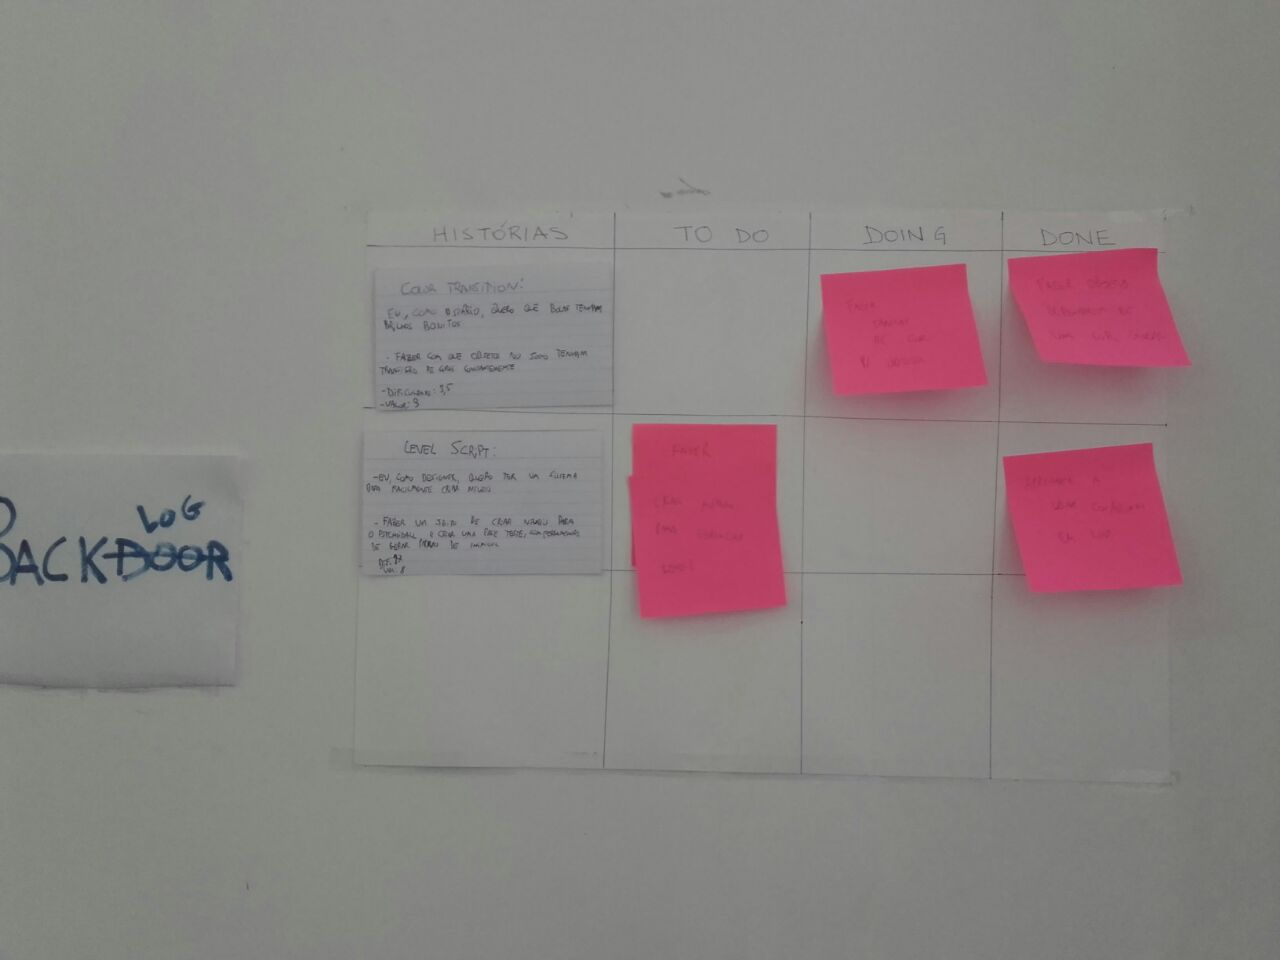
\includegraphics[scale=.3]{kanban}
\centering
\caption{Kanban utilizado durante o desenvolvimento de \textit{PsyChO: The Ball}}
\end{figure}

Entretanto, após alguns meses utilizando essa técnica, o tempo gasto em sua manutenção acabou se tornando mais trabalhoso do que produtivo para o projeto e seu uso foi decaindo. Desta forma o \textit{Kanban} foi substituido por várias pequenas técnicas ágeis, como lançamentos frequentes do jogo, \textit{sprints} (onde era determinado um prazo de uma ou duas semanas para terminar funcionalidades no jogo) e constantes re-avaliações com consulta de \textit{feedback}.

Por último, uma técnica muito presente no desenvolvimento do jogo foi a utilização de documentação para marcar mudanças e melhorias no projeto. Os dois documento mais importantes são o \textit{DEVLOG}\footnote{https://github.com/uspgamedev/Project-Telos/blob/dev/docs/DEVLOG.md} e \textit{CHANGELOG}\footnote{https://github.com/uspgamedev/Project-Telos/blob/dev/docs/CHANGELOG.md}. O \textit{DEVLOG} foi um necessário para mostrar o progresso e tempo gasto no projeto, enquanto este fazia parte da disciplina \textit{MAC0214 Atividade Curricular em Cultura e Extensão}. Nele existem várias entradas detalhando atividades feitas no jogo durante o desenvolvimento. O \textit{CHANGELOG} por outro lado serve para marcar lançamentos do jogo, descrevendo \textit{features} novos adicionados em cada \textit{sprint} feito. Ambos documentos foram de grande utilidade no início do desenvolvimento de \textit{PsyChO: The Ball}, pois exibem concretamente o fluxo de progresso na criação do jogo.

% ---------------------------------------------------------------------------- %
\section{Ferramentas}
\label{sec:ferramentas}

Uma das escolhas feitas para o desenvolvimento de \textit{PsyChO: The Ball} foi a utilização exclusiva de \textit{Software Livre}. Essa decisão se deu tanto pela liberdade que essas ferramentas permitem em sua utilização, quanto pelo objetivo de incentivar mais o uso desse tipo de software, mostrando que é tão eficiente quanto o uso de software proprietário. Assim, como critério de escolha para cada área de desenvolvimento do jogo, foi determinado algum software livre que tenha uma comunidade ativa (para a solução de problemas e disponibilidade de bibliotecas), constante atualização de suas funcionalidades, versões estáveis e uma recomendação de seu uso no desenvolvimento de jogos.

O arcabouço utilizado no desenvolvimento de \textit{PsyChO: The Ball} foi a \textit{Love2d} ou \textit{LÖVE}\footnote{https://love2d.org/}, uma \textit{framework} gratuita que utiliza a linguagem \textit{Lua}\footnote{https://www.lua.org/portugues.html}.

Como sistema de controle de versão foi utilizado \textit{Git}\footnote{https://git-scm.com/} através da plataforma de uso grátis \textit{Github}\footnote{https://github.com/}.

Para a produção de música foi utilizado \textit{LMMS}\footnote{https://lmms.io/}, um software livre gratuito para manipulação e criação de sons.

Por último, para manipulação de imagens, foi utilizada a ferramenta \textit{Gimp}\footnote{https://www.gimp.org/}.

\begin{figure}[h!]

\includegraphics[scale=.5]{icons}
\centering
\caption{Da esquerda pra direita, ícones de \textit{LÖVE}, \textit{Lua}, \textit{Git}, \textit{Github}, \textit{LMMS} e \textit{Gimp}}
\end{figure}

Dentre essas ferramentas, vale ressaltar um ponto muito interessante do arcabouço \textit{LÖVE}: seu \textit{gameloop} tem o diferencial de deslocar todas as verificações de \textit{input} do usuário como \textit{callbacks assíncronos}. Estes são funções que a própria \textit{framework} vai chamar quando ocorrer algum \textit{input} do usuário, como quando ele pressionar um botão do teclado ou mover o mouse. Através de subrotinas, o arcabouço está constantemente aguardando sinais que ativem essas funções e assim o desenvolvedor não precisa se preocupar em lidar com otimização ou código confuso na hora de esperar e tratar comandos dados pelo usuário. Isso foi uma grande vantagem que determinou a escolha dessa ferramenta na produção de \textit{PsyChO: The Ball}.

% ---------------------------------------------------------------------------- %
